The clustering algorithms used for the SmartEater data set, were DBSCAN and OPTICS. One of the advantages of these density-based clustering methods (as mentioned in section \ref{section:densityBasedMethods}) are that there are less parameters to configure. Another reason for choosing these methods, is that there is no need to define a fixed number of \textit{k} clusters to find, since the cluster boundaries are regulated by density. This technique also allows to arbitrary-shaped clusters to be correctly identified.

\subsubsection{DBSCAN}
Section \ref{section:DBSCAN}...
One of the disadvantages of DBSCAN, is the need to specify parameters, which can change the outcome of the results. In order to establish suitable parameters, k-dist graphs generated for the 1h and 3h data sets. The graphs contained the distances to the k nearest neihbors. As recommended by \textcite{DBSCAN}[230], MinPts and \textit{k} were set to 4 and the graphs were used to determine Eps. The idea is to select Eps suitable for the "thinnest" cluster, however being careful to avoid noise. As can be seen in figures \ref{figure:kDistGraphDBSCAN1h} and \ref{figure:kDistGraphDBSCAN3h}, the valley starts at roughly a 4th nearest neighbor distance of 2. 



\begin{figure*}[h]
  \centering
  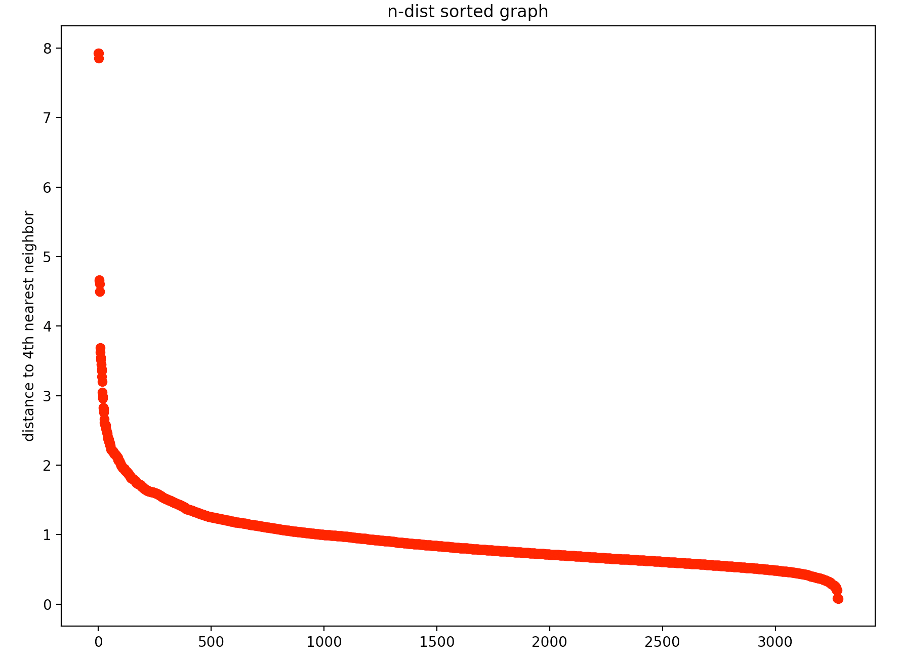
\includegraphics[width=0.5\textwidth]{./images/kDistGraphDBSCAN1h.png}
  \caption{Sorted 4-dist graph of the 3h data set (distance for each point to its fourth nearest neighbor). The valley starts at roughly the 4th nearest neighbor distance of 2.}
  \label{figure:kDistGraphDBSCAN1h}
\end{figure*}

\begin{figure*}[h]
  \centering
  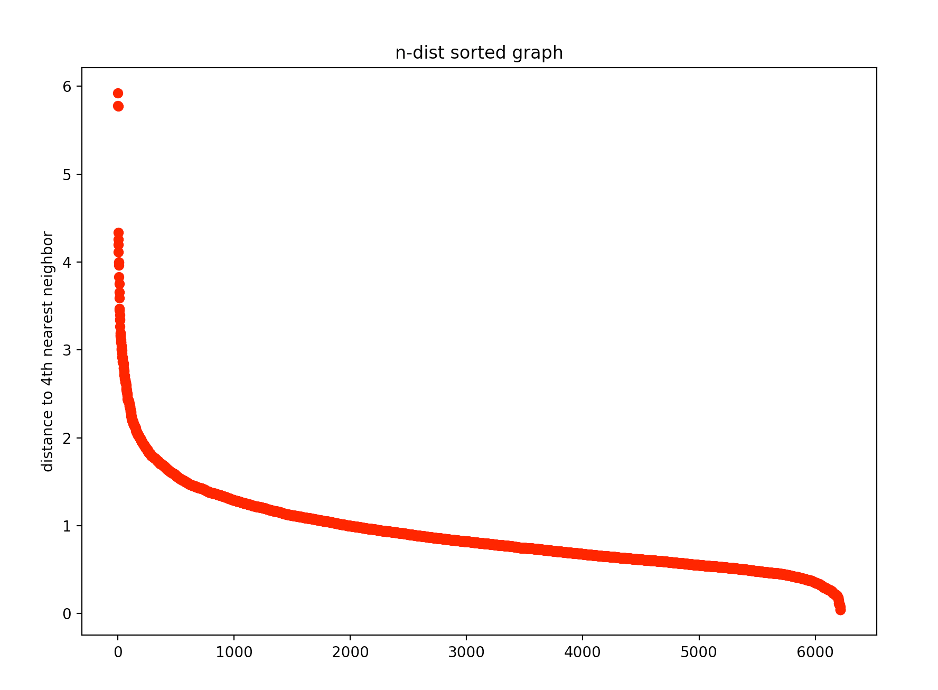
\includegraphics[width=0.5\textwidth]{./images/kDistGraphDBSCAN3h.png}
  \caption{Sorted 4-dist graph of the 1h data set (distance for each point to its fourth nearest neighbor). The valley starts at roughly the 4th nearest neighbor distance of 2.}
  \label{figure:kDistGraphDBSCAN3h}
\end{figure*}


% \begin{figure}
%   \centering
%   \parbox{5cm}{
%     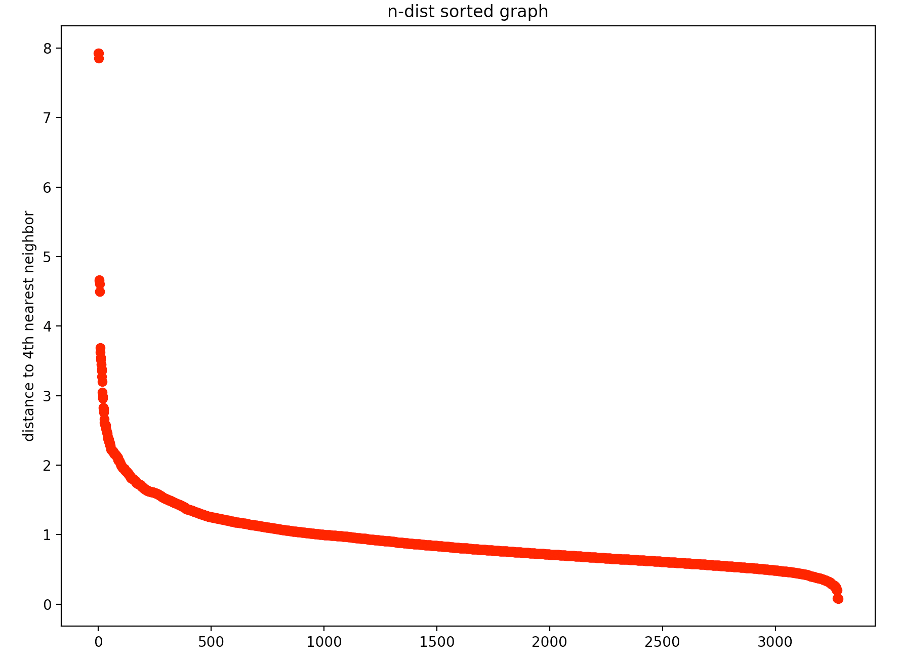
\includegraphics[width=0.5\textwidth]{./images/kDistGraphDBSCAN1h.png}
%       \caption{1h data set}
%       \label{figure:kDistGraphDBSCAN1h}
%   \qquad
%   \begin{minipage}{5cm}

%       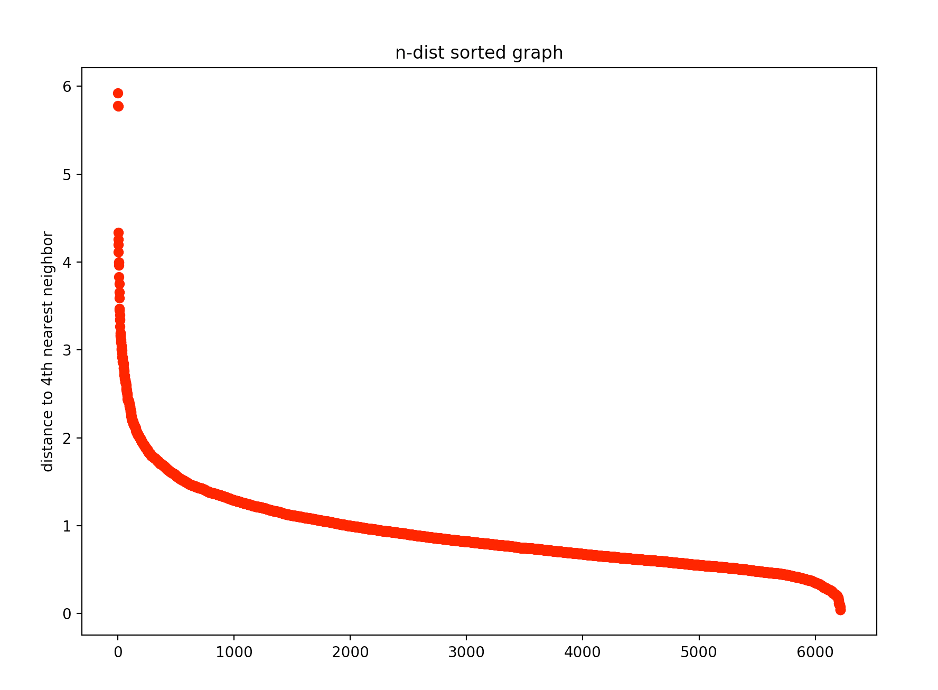
\includegraphics[width=0.5\textwidth]{./images/kDistGraphDBSCAN3h.png}
%       \caption{3h data set}
%       \label{figure:kDistGraphDBSCAN3h}
%   \end{minipage}
%   \end{figure}



% \begin{figure}
%   \centering
%   \begin{subfigure}[b]{0.5\textwidth}
%       \centering
%       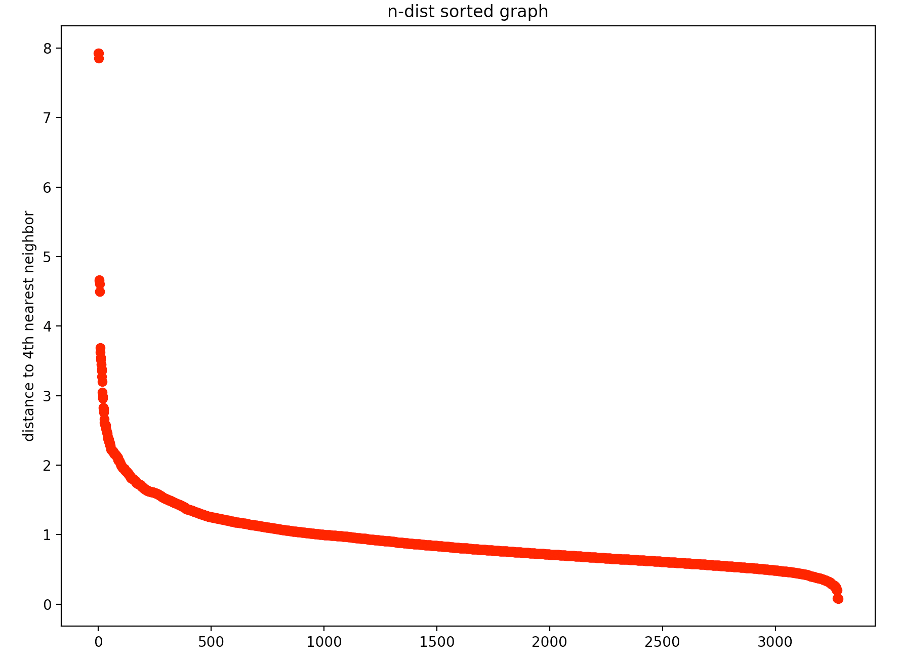
\includegraphics[width=0.5\textwidth]{./images/kDistGraphDBSCAN1h.png}
%       \caption{Sorted 4-dist graph of the 3h data set (distance for each point to its fourth nearest neighbor). The valley starts at roughly the 4th nearest neighbor distance of 2.}
%       \label{figure:kDistGraphDBSCAN1h}
%   \end{subfigure}
%   \hfill
%   \begin{subfigure}[b]{0.5\textwidth}
%       \centering
%       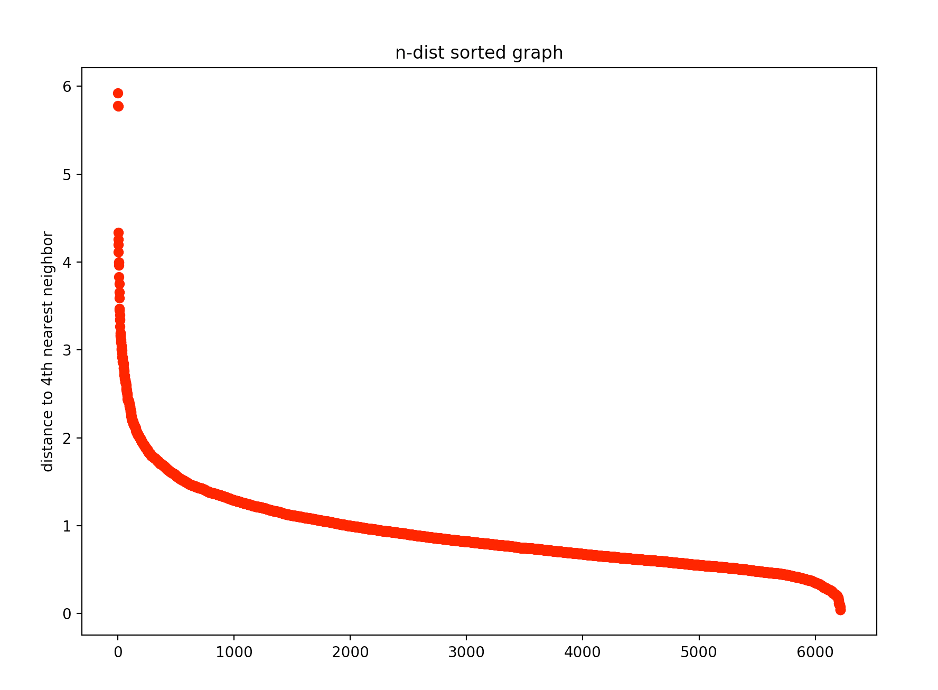
\includegraphics[width=0.5\textwidth]{./images/kDistGraphDBSCAN3h.png}
%       \caption{Sorted 4-dist graph of the 1h data set (distance for each point to its fourth nearest neighbor). The valley starts at roughly the 4th nearest neighbor distance of 2.}
%       \label{figure:kDistGraphDBSCAN3h}
%   \end{subfigure}
  
%   \caption{Sorted 4-dist graphs (distance for each point to its fourth nearest neighbor), used to determine a suitable Eps parameter for the DBSCAN algorithm. The valley starts at roughly the 4th nearest neighbor distance of 2, therefore Eps should be 2.}
%   \label{figure:kDistGraphDBSCAN}
% \end{figure}

% \begin{figure}
%   \centering
%   \begin{subfigure}{.5\textwidth}
%     \centering
%     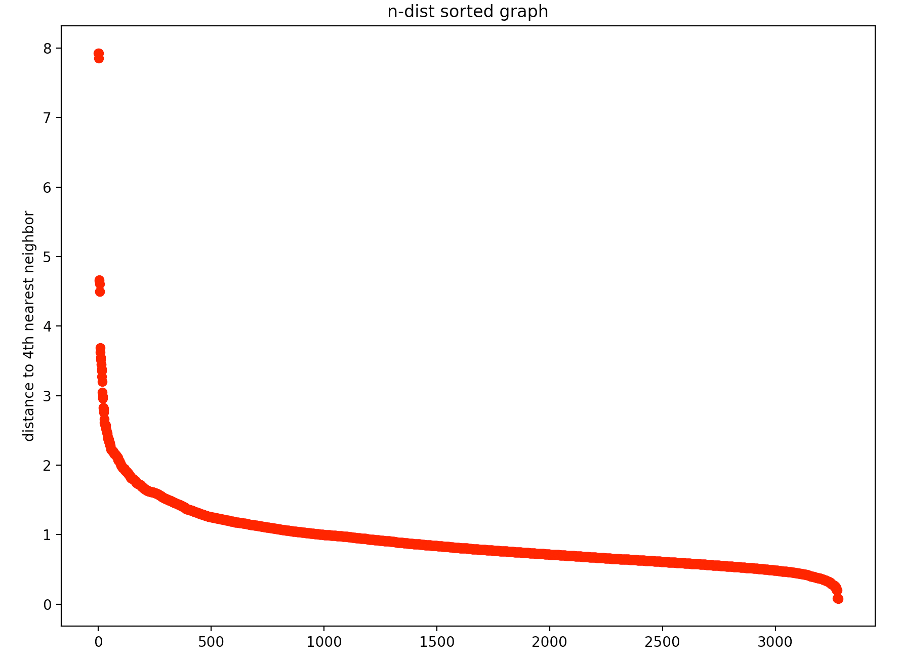
\includegraphics[width=0.5\textwidth]{./images/kDistGraphDBSCAN1h.png}
%   \caption{1h dataset}
%   \label{figure:kDistGraphDBSCAN1h}
%   \end{subfigure}%
%   \begin{subfigure}{.5\textwidth}
%     \centering
%     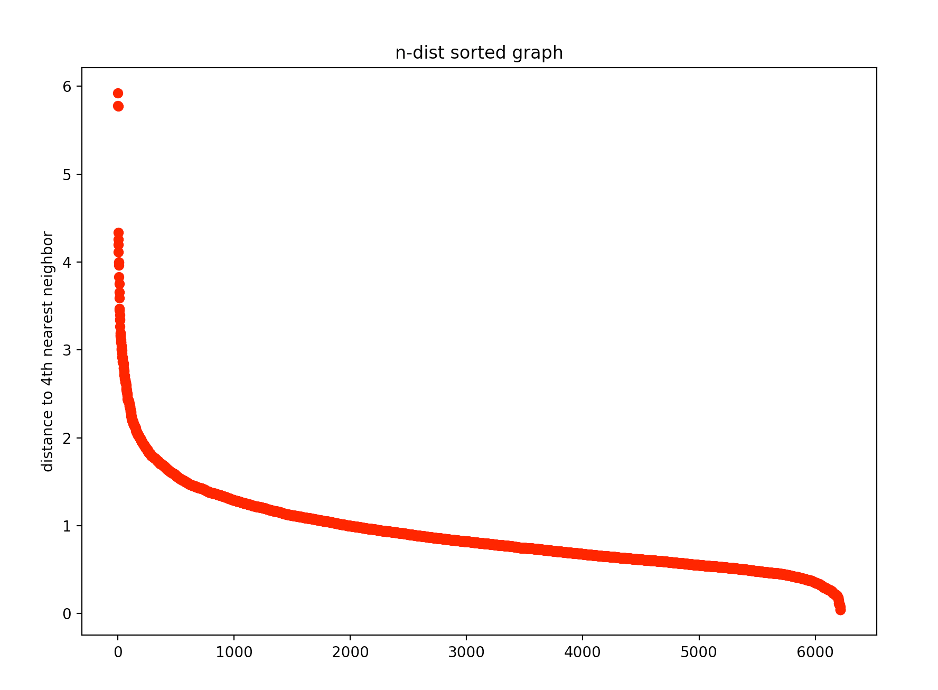
\includegraphics[width=0.5\textwidth]{./images/kDistGraphDBSCAN3h.png}
%     \caption{3h data set}
%     \label{figure:kDistGraphDBSCAN3h}
%   \end{subfigure}
%   \caption{Sorted 4-dist graphs (distance for each point to its fourth nearest neighbor), used to determine a suitable Eps parameter for the DBSCAN algorithm. The valley starts at roughly the 4th nearest neighbor distance of 2, therefore Eps should be 2.}
%   \label{figure:kDistGraphDBSCAN}
%   \end{figure}



  


\subsubsection{OPTICS}








%---------

Since density based algorithms do not require specifying a number of clusters in advance

\& clusters can be of any shape

optics: two options: xi (automatic technique from \textcite{OPTICS}, or dbscan)


